%%%%%%%%%%%%%%%%%%%%%%%%%%%%%%%%%%%%%%%%%
% FRI Data Science_report LaTeX Template
% Version 1.0 (28/1/2020)
% 
% Jure Demšar (jure.demsar@fri.uni-lj.si)
%
% Based on MicromouseSymp article template by:
% Mathias Legrand (legrand.mathias@gmail.com) 
% With extensive modifications by:
% Antonio Valente (antonio.luis.valente@gmail.com)
%
% License:
% CC BY-NC-SA 3.0 (http://creativecommons.org/licenses/by-nc-sa/3.0/)
%
%%%%%%%%%%%%%%%%%%%%%%%%%%%%%%%%%%%%%%%%%


%----------------------------------------------------------------------------------------
%	PACKAGES AND OTHER DOCUMENT CONFIGURATIONS
%----------------------------------------------------------------------------------------
\documentclass[fleqn,moreauthors,10pt]{ds_report}
\usepackage[english]{babel}

\graphicspath{{fig/}}




%----------------------------------------------------------------------------------------
%	ARTICLE INFORMATION
%----------------------------------------------------------------------------------------

% Header
\JournalInfo{FRI Natural language processing course 2025}

% Interim or final report
\Archive{Project report} 
%\Archive{Final report} 

% Article title
\PaperTitle{'; DROP TABLE TEAMS; --} 

% Authors (student competitors) and their info
\Authors{Henri Sellis, Igor Sitek}

% Advisors
\affiliation{\textit{Advisors: Aleš Žagar}}

% Keywords
\Keywords{Retrieval-Augmented Generation, RAG, web scraping, rank algorithms, Python, keyword extraction}
\newcommand{\keywordname}{Keywords}


%----------------------------------------------------------------------------------------
%	ABSTRACT
%----------------------------------------------------------------------------------------

\Abstract{
For our Natural Language Processing course group project, we are developing a conversational agent that retrieves additional information from Google Scholar documents, to increase the quality of answering questions, ensuring up-to-date outputs. To accomplish this, first a number of most relevant tags are extracted from the user input, then corresponding queries are made to retrieve documents from Google Scholar, and finally the documents, alongside with the original user input, are passed to a Large Language Model, to generate a paraphrased response.
}

%----------------------------------------------------------------------------------------

\begin{document}

% Makes all text pages the same height
\flushbottom 

% Print the title and abstract box
\maketitle 

% Removes page numbering from the first page
\thispagestyle{empty} 

%----------------------------------------------------------------------------------------
%	ARTICLE CONTENTS
%----------------------------------------------------------------------------------------

\section*{Introduction}
	Large Language Models have proven to be very successful at general-knowledge topics, but a trained model cannot continuously stay up to date with the most recent academic topics. To solve this problem, we are using Retrieval-Augmented Generation to provide an LLM with the most relevant academic papers to allow the LLM to generate more relevant and accurate responses. The documents are retrieved from Google Scholar, as it is an easily accessible repository with lots of academic papers.
	
	With the increasing number of scientific papers published across the world, it is difficult to analyze the most relevant data. Automated literature lookup based on relevant datasets might highly improve the process of conducting scientific experiments, mitigating the risk of work duplication. However, it is crucial to ensure up-to-date answers, thus relying on static datasets is not the most optimal approach. RAG-augmented query analyses alongside with web crawling and web scraping techniques seem to be promising to resolve that matter.


%------------------------------------------------

\section*{Methodology}

\begin{figure*}[ht]\centering 
	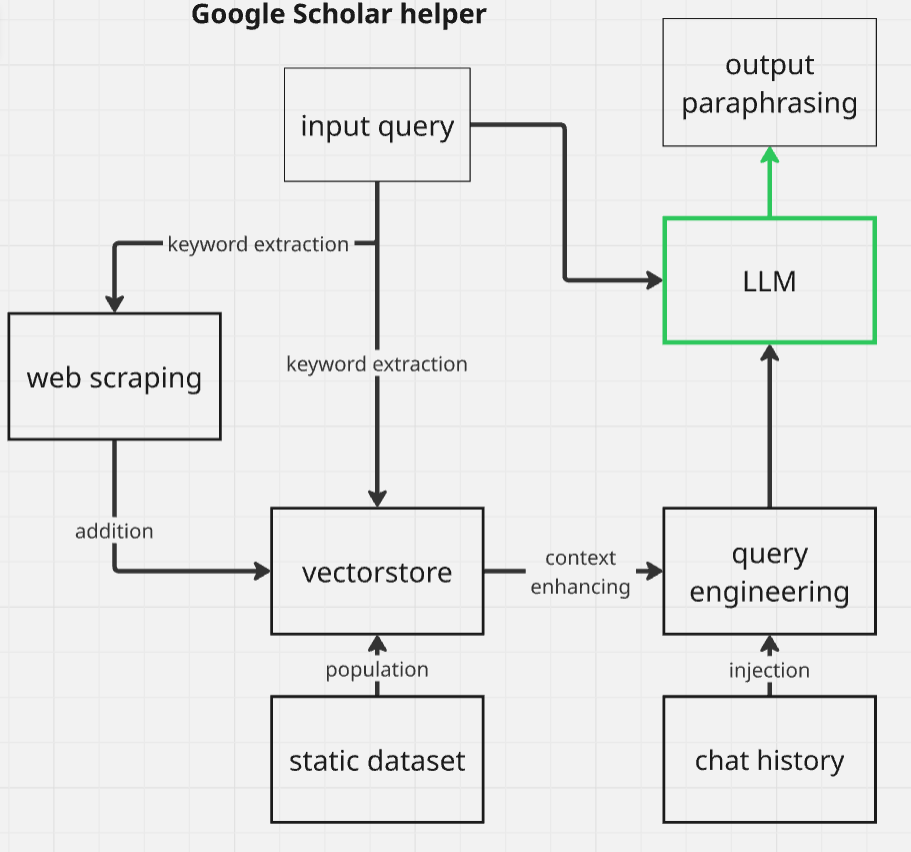
\includegraphics[width=0.7\linewidth]{images/scheme.png}
	\caption{\textbf{System scheme} High-level overview of chat-bot system proposed in this paper.}
	\label{fig:scheme}
\end{figure*}

The proposed methodology scheme is presented on figure~\ref{fig:scheme}. Each vital step is descibed in the following subsections of this article.

\subsection*{Keyword extraction}

In order to be able to provide relevant literature, our approach focuses on keyword extraction both from scientific papers and user input. This enables us to create a lookup in available works that would be further parsed.

To further specify our domain, we will limit this research to English papers only, eliminating the necessity of language-independent vector transitions and specific rules in different languages. The English was chosen as it is the most popular language with the highest amount of data available, and it is characterized by low sentence sensitivity (in opposition to romance languages). That characteristic enables low-effort word stemming in text processing~\cite{turney2000learning}.

Work ~\cite{siddiqi2015keyword} is a review of existing methods for keyword extraction, containing summaries of different supervised and unsupervised algorithms. Upon these, Neural Networks seem to be used mainly. On the other hand, ready-to-use implementations of RAKE and RANK algorithms (like TextRank~\cite{textrank} - https://github.com/davidadamojr/TextRank or TopicRank~\cite{bougouin2013topicrank} - https://github.com/Aayushpatel007/topicrankpy) seem to be useful enough for our case. Further training using these algorithms will be conducted with relevant datasets.

Model evaluation and learning rate will be measured by the statistical indicators as proposed in work~\cite{firoozeh2020keyword}: these include TF-IDF, co-occurrence, and similarity-based values.

\subsection*{Corpus analysis}

Following datasets were found in order to fine-tune existing algorithms:

\begin{itemize}
    \item https://github.com/SDuari/Keyword-Extraction-Datasets,
    \item https://github.com/LIAAD/KeywordExtractor-Datasets,
    \item https://github.com/boudinfl/ake-datasets,
\end{itemize}

All of them consist of zip folders with two sub-folders, one containing whole papers in TXT format, and one with manually gathered keywords and key-phrases. These files are matched based on a common key - included in the filename.

\subsection*{Keyword lookup}

After parsing user input and resolving its keywords, the next step consists of static dataset lookup in order to find relevant papers. The algorithm is yet to be specified - whereas Levenshtein distance~\cite{yujian2007normalized} might be useful, it will probably not be enough since multiple subsets of keywords will be searched for.

\subsection*{Web scraping}

Provided keywords and user input are combined into a suitable Google Scholar query, in order to assure up-to-date answers. Script is going to be implemented in Python language, using one of the open-source web-scraping packages.
\newline
Having in mind commonly used firewalls on publisher websites, some tools like Sci-Hub are considered to bypass them and streamline the process of data scraping. Knowledge must be free!

\subsection*{Data combining and paraphrasing}

All the relevant documents (found in the dataset and downloaded from the web) are going to be combined with user input and passed into a pre-trained LLM model. Multiple open-source models will be tested and manually validated. Fine-tuning the LLM model and prompt engineering techniques should provide a satisfactory and reliable output to the user.

% \begin{figure}[ht]\centering
% 	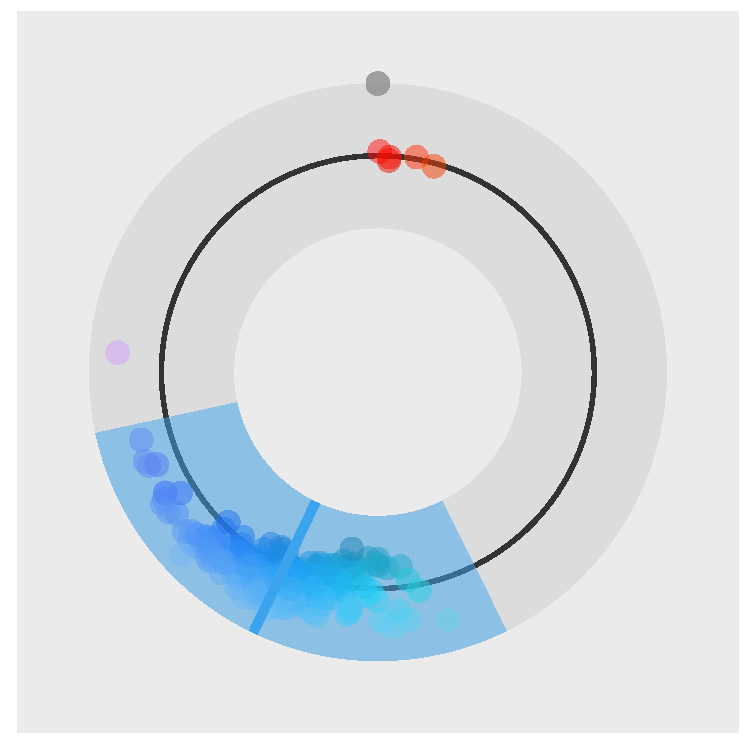
\includegraphics[width=\linewidth]{images/single_column.pdf}
% 	\caption{\textbf{A random visualization.} This is an example of a figure that spans only across one of the two columns.}
% 	\label{fig:column}
% \end{figure}

% % \begin{figure*} makes the figure take up the entire width of the page
% \begin{figure*}[ht]\centering 
% 	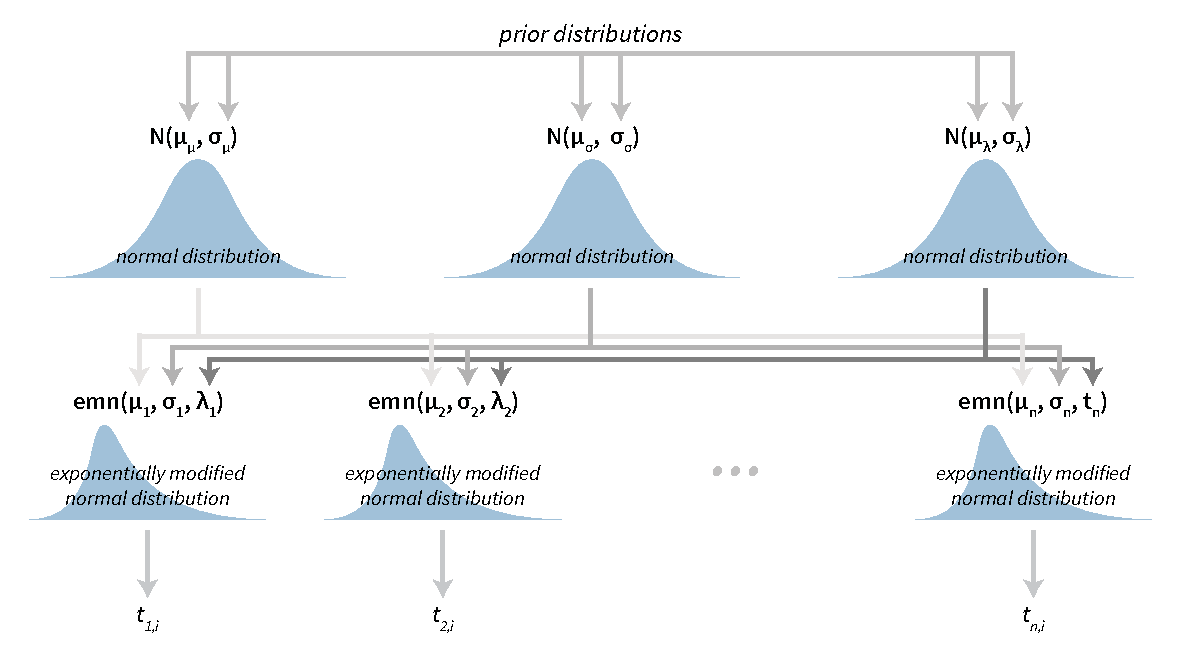
\includegraphics[width=\linewidth]{images/whole_page.pdf}
% 	\caption{\textbf{Visualization of a Bayesian hierarchical model.} This is an example of a figure that spans the whole width of the report.}
% 	\label{fig:whole}
% \end{figure*}


\

%----------------------------------------------------------------------------------------
%	REFERENCE LIST
%----------------------------------------------------------------------------------------
\bibliographystyle{unsrt}
\bibliography{report}


\end{document}